\section{Problem Introduction}
\label{sec:introduction}

This report is concerned with finding a good scheduling approach for a given set of tasks (todos) with duration, priority, location and due date.
The software attached with this report, going by the name of \textit{Melon}, consists of two parts: the \texttt{melon} task scheduling package itself and the Graphical User Interface written using the Qt6 framework, contained in \texttt{melongui}.
Both of these are published as a package \textbf{melon-scheduler}, available \href{https://pypi.org/project/melon-scheduler/}{on PyPi}. It may be installed using

\bashblock{pip install melon-scheduler}
for just the scheduler, without the \gls{gui},

\bashblock{pip install melon-scheduler[gui]} with the \gls{gui} or optionally,

\bashblock{pip install melon-scheduler[gui,plots,numba]} with all extras.

The package is capable of downloading and synchronising tasks from a calendar server supporting the industry-standard CalDAV protocol, displaying and editing them in the \gls{gui} and finally scheduling them into a calendar (cf. \Cref{fig:calendar}).
The scheduling mechanism we implemented is a \gls{mcmc} method.

\begin{figure}[H]
  \centering
  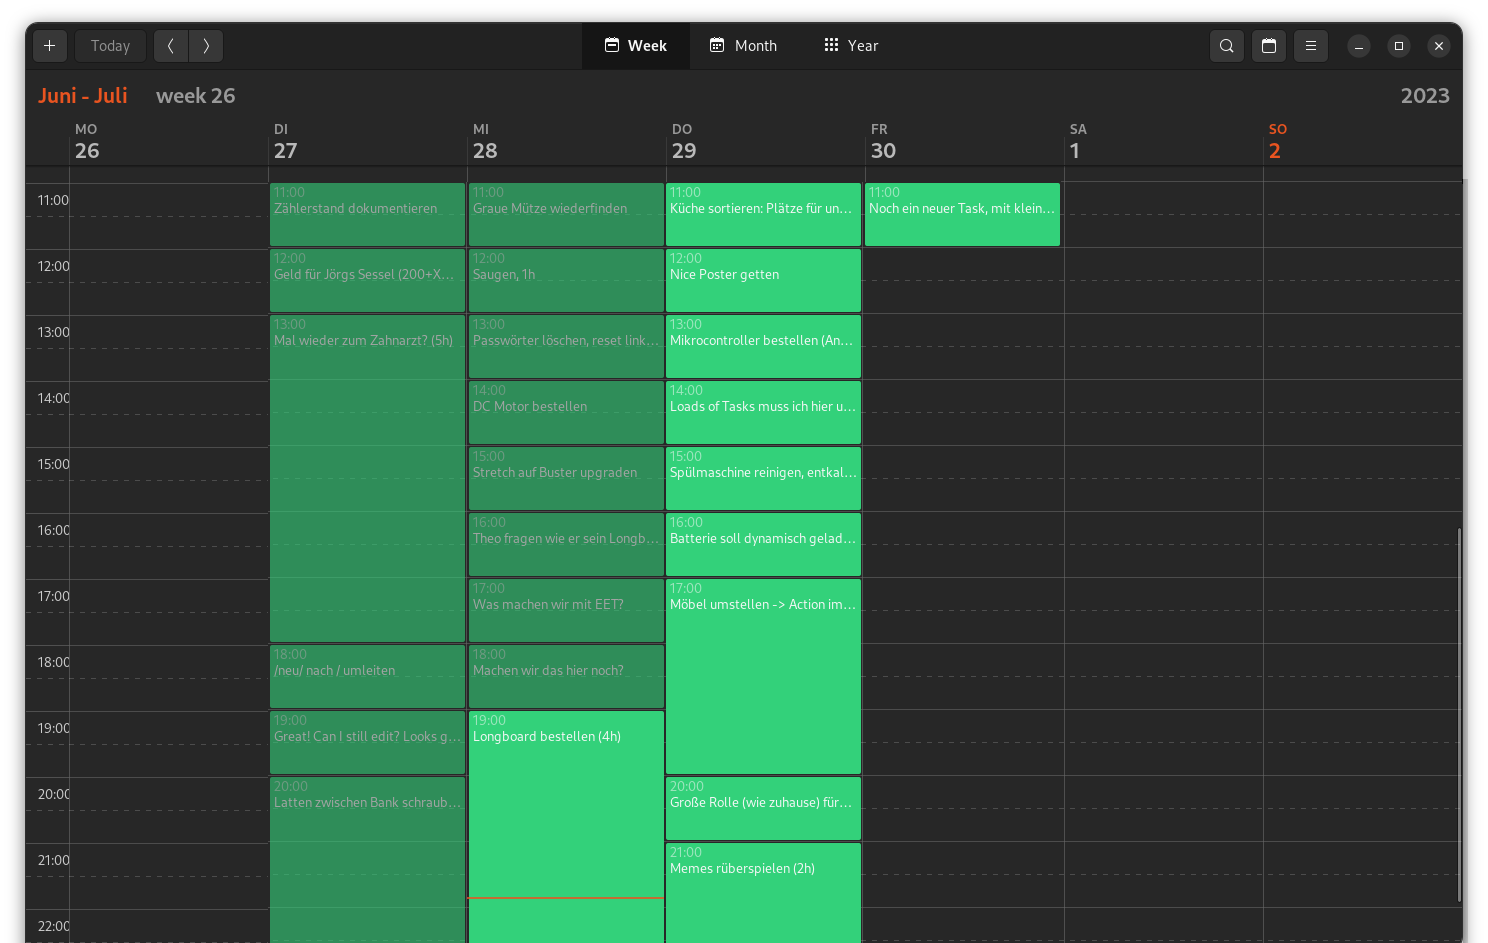
\includegraphics[width=\linewidth]{figures/exported-calendar.png}
  \caption{The scheduled tasks, as displayed in \textit{Gnome Calendar} (the default duration for each task is one hour). Theoretically existent events could be taken into account for task scheduling as well, just as well as breaks.}
  \label{fig:calendar}
\end{figure}

\subsection{Idea of the Algorithm}
We work with the following assumption on the state: the entire scheduling, given the set of tasks, is solely determined by the order in which the tasks are scheduled.
That is, for a given order of tasks, the full schedule can be created using the supplied input data.
With this assumption, finding the absolute optimum is tedious, especially for a large number of tasks $N \gg 1$, as there are $N!$ possible ways to order the tasks.

The idea of the Monte Carlo method implemented here is to minimise a penalty function (borrowing the term \textit{energy} from physics) over the discrete state space of size $\mathcal{O}(N!)$ using a stochastic approach, as sketched in \Cref{sec:theory}.
The four key properties we aim to optimise for are:
\begin{itemize}
  \tightlist
  \item spending a minimal amount of time to complete all tasks,
  \item scheduling high priority tasks first,
  \item a low number of commutes between locations and
  \item having all tasks completed on time.
\end{itemize}
Due to this choice of state representation, the problem broadly mimics a Traveling Salesman Problem.
